\documentclass[tikz,border=10pt]{standalone}
\usepackage[utf8]{inputenc}
\usepackage{tikz}
\usetikzlibrary{shapes,arrows.meta,positioning,calc,fit}

\definecolor{ScoutGreen}{HTML}{005432}
\definecolor{ScoutNavy}{HTML}{002855}
\definecolor{ScoutBlue}{HTML}{006EB6}
\definecolor{ScoutRed}{HTML}{A31920}
\definecolor{ScoutAmber}{HTML}{D97706}
\definecolor{BorderGray}{HTML}{CBD5E1}

\begin{document}
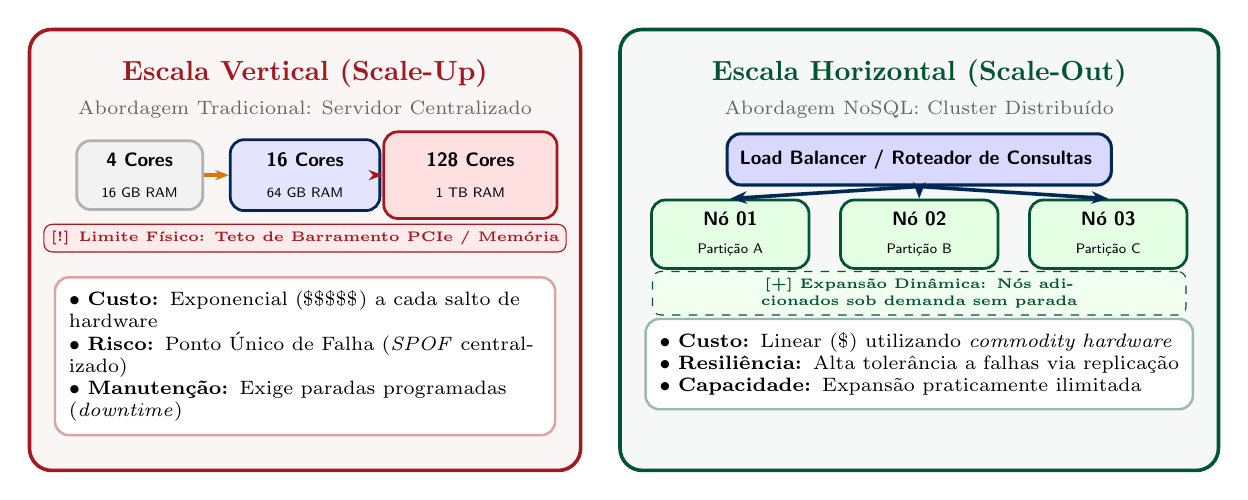
\begin{tikzpicture}[
    font=\sffamily,
    panel/.style={draw=#1, rounded corners=8pt, fill=#1!4, line width=1.3pt, inner sep=8pt},
    serverbox/.style={draw=BorderGray, rounded corners=5pt, fill=white, line width=1pt, align=center, inner sep=4.5pt},
    arrow/.style={-{Stealth[length=6pt]}, line width=1.3pt}
]

  % -------------------------------------------------------------
  % PAINEL ESQUERDO: ESCALA VERTICAL (SCALE-UP)
  % -------------------------------------------------------------
  \node[panel=ScoutRed, minimum width=7.0cm, minimum height=5.6cm] (p_vert) at (0, 0) {};
  \node[font=\bfseries\normalsize, text=ScoutRed, anchor=north] at (p_vert.north) [yshift=-8pt] {Escala Vertical (Scale-Up)};
  \node[font=\scriptsize, text=gray!80!black, anchor=north] at (p_vert.north) [yshift=-23pt] {Abordagem Tradicional: Servidor Centralizado};

  % Servidores em progressão
  \node[serverbox, draw=gray!60, fill=gray!10, minimum width=1.6cm, minimum height=0.75cm] (srv1) at (-2.1, 0.95) {
    \scriptsize \textbf{4 Cores}\\[-1pt]\tiny 16 GB RAM
  };
  \node[serverbox, draw=ScoutNavy, fill=blue!10, minimum width=1.9cm, minimum height=0.9cm] (srv2) at (0.0, 0.95) {
    \scriptsize \textbf{16 Cores}\\[-1pt]\tiny 64 GB RAM
  };
  \node[serverbox, draw=ScoutRed, fill=red!12, minimum width=2.2cm, minimum height=1.1cm] (srv3) at (2.1, 0.95) {
    \scriptsize \textbf{128 Cores}\\[-1pt]\tiny 1 TB RAM
  };

  \draw[-{Stealth[length=5pt]}, line width=1.4pt, color=ScoutAmber] (srv1) -- (srv2);
  \draw[-{Stealth[length=5pt]}, line width=1.4pt, color=ScoutRed] (srv2) -- (srv3);

  % Teto Físico
  \draw[dashed, line width=1.2pt, color=ScoutRed] (-3.1, 0.15) -- (3.1, 0.15);
  \node[fill=red!8, draw=ScoutRed, rounded corners=3pt, inner sep=2.5pt, font=\tiny\bfseries, text=ScoutRed] at (0, 0.15) {
    [!] Limite Físico: Teto de Barramento PCIe / Memória
  };

  % Resumo Scale-Up (totalmente contido com text width)
  \node[draw=ScoutRed!40, fill=white, rounded corners=5pt, font=\scriptsize, align=left, inner sep=5pt, line width=0.9pt, text width=6.0cm] at (0, -1.35) {
    $\bullet$ \textbf{Custo:} Exponencial (\$\$\$\$\$) a cada salto de hardware\\
    $\bullet$ \textbf{Risco:} Ponto Único de Falha (\textit{SPOF} centralizado)\\
    $\bullet$ \textbf{Manutenção:} Exige paradas programadas (\textit{downtime})
  };

  % -------------------------------------------------------------
  % PAINEL DIREITO: ESCALA HORIZONTAL (SCALE-OUT)
  % -------------------------------------------------------------
  \node[panel=ScoutGreen, minimum width=7.6cm, minimum height=5.6cm] (p_horiz) at (7.8, 0) {};
  \node[font=\bfseries\normalsize, text=ScoutGreen, anchor=north] at (p_horiz.north) [yshift=-8pt] {Escala Horizontal (Scale-Out)};
  \node[font=\scriptsize, text=gray!80!black, anchor=north] at (p_horiz.north) [yshift=-23pt] {Abordagem NoSQL: Cluster Distribuído};

  % Load Balancer
  \node[serverbox, draw=ScoutNavy, fill=blue!15, line width=1.1pt, minimum width=4.2cm, minimum height=0.65cm] (lb) at (7.8, 1.15) {
    \scriptsize \textbf{Load Balancer / Roteador de Consultas}
  };

  % Nós em cluster
  \node[serverbox, draw=ScoutGreen, fill=green!10, minimum width=2.0cm] (n1) at (5.4, 0.2) {
    \scriptsize \textbf{Nó 01}\\[-2pt]\tiny Partição A
  };
  \node[serverbox, draw=ScoutGreen, fill=green!10, minimum width=2.0cm] (n2) at (7.8, 0.2) {
    \scriptsize \textbf{Nó 02}\\[-2pt]\tiny Partição B
  };
  \node[serverbox, draw=ScoutGreen, fill=green!10, minimum width=2.0cm] (n3) at (10.2, 0.2) {
    \scriptsize \textbf{Nó 03}\\[-2pt]\tiny Partição C
  };

  \draw[arrow, color=ScoutNavy] (lb.south) -- (n1.north);
  \draw[arrow, color=ScoutNavy] (lb.south) -- (n2.north);
  \draw[arrow, color=ScoutNavy] (lb.south) -- (n3.north);

  % Nota elástica (contida)
  \node[draw=ScoutGreen, dashed, fill=green!6, rounded corners=3pt, font=\tiny\bfseries, text=ScoutGreen, inner sep=2.5pt, align=center, text width=6.6cm] at (7.8, -0.55) {
    [+] Expansão Dinâmica: Nós adicionados sob demanda sem parada
  };

  % Resumo Scale-Out (totalmente contido com text width)
  \node[draw=ScoutGreen!40, fill=white, rounded corners=5pt, font=\scriptsize, align=left, inner sep=5pt, line width=0.9pt, text width=6.6cm] at (7.8, -1.45) {
    $\bullet$ \textbf{Custo:} Linear (\$) utilizando \textit{commodity hardware}\\
    $\bullet$ \textbf{Resiliência:} Alta tolerância a falhas via replicação\\
    $\bullet$ \textbf{Capacidade:} Expansão praticamente ilimitada
  };

\end{tikzpicture}
\end{document}
